%% This is file `sample-sigconf.tex',
%% generated with the docstrip utility.
%%
%% The source files were:
%%
%% samples.dtx  (with options: `sigconf')
% TODO: Add review at the end
\documentclass[sigconf]{acmart}
%% \BibTeX command to typeset BibTeX logo in the docs
\AtBeginDocument{%
  \providecommand\BibTeX{{%
    \normalfont B\kern-0.5em{\scshape i\kern-0.25em b}\kern-0.8em\TeX}}}

%% Rights management information.  This information is sent to you
%% when you complete the rights form.  These commands have SAMPLE
%% values in them; it is your responsibility as an author to replace
%% the commands and values with those provided to you when you
%% complete the rights form.
\setcopyright{acmcopyright}
\copyrightyear{2024}
\acmYear{2024}
\acmDOI{XXXXXXX.XXXXXXX}

\acmConference[ICSE 2024]{46th International Conference on Software Engineering}{April 2024}{Lisbon, Portugal}

%%
%% end of the preamble, the start of the body of the document source.
\begin{document}

%%
%% The "title" command has an optional parameter,
%% allowing the author to define a "short title" in page headers.
\title{Implementing the Visual Debugger: Past, Present, and Future}

\author{Tim Kr\"{a}uter}
\email{tkra@hvl.no}
\orcid{0000-0003-1795-0611}
\affiliation{
  \institution{Western Norway University of Applied Sciences}
  \city{Bergen}
  \country{Norway}
}

\author{Patrick Stünkel}
\email{patrick.stuenkel@hvl.no}
\orcid{0000-0002-0537-295X}
\affiliation{
  \institution{Western Norway University of Applied Sciences}
  \city{Bergen}
  \country{Norway}
}

\author{Adrian Rutle}
\email{aru@hvl.no}
\orcid{0000-0002-4158-1644}
\affiliation{
  \institution{Western Norway University of Applied Sciences}
  \city{Bergen}
  \country{Norway}
}

\author{Yngve Lamo}
\email{yla@hvl.no}
\orcid{0000-0001-9196-1779}
\affiliation{
  \institution{Western Norway University of Applied Sciences}
  \city{Bergen}
  \country{Norway}
}

\renewcommand{\shortauthors}{Kräuter et al.}
\newcommand{\intellij}{IntelliJ IDEA}
% Four pages + 1 page of references.

\begin{abstract}
    % One sentence tool description
    The visual debugger is an IntelliJ IDEA plugin that presents debug information as an object diagram for improved program understanding.
    % Past: Lessons learned and roadblocks + experience
    Remembering our \textit{past} development, we detail the lessons learned and roadblocks we have experienced while implementing and integrating the visual debugger into IntelliJ IDEA.
    % Present: New features and improvements
    Furthermore, we describe recent improvements and new features added to the visual debugger, greatly improving the plugin in the \textit{present}.
    % Future: possible solutions to the roadblocks and future work
    Looking into the \textit{future}, we propose solutions to overcome the roadblocks encountered during plugin development and further plans for the visual debugger.
\end{abstract}

\begin{CCSXML}
<ccs2012>
   <concept>
       <concept_id>10011007.10011006.10011066.10011069</concept_id>
       <concept_desc>Software and its engineering~Integrated and visual development environments</concept_desc>
       <concept_significance>500</concept_significance>
       </concept>
 </ccs2012>
\end{CCSXML}

\ccsdesc[500]{Software and its engineering~Integrated and visual development environments}

\keywords{Debugging, Visual Debugging, IDE plugin, IDE Integration}

% Fitting topics from the workshop:
% 1. The development of plugins, add-ons, and extensions for IDEs.
% 2. Visualizations in the IDEs.
% 3. Anecdotal experience about why a certain tool or research approach was not implemented on top of the IDE infrastructure, but researchers chose alternatives (e.g., a CLI tool), what the blockers were, and how the IDEs can improve to become more convenient for prototyping.

\received{7 December 2023}
% \received[revised]{7 December 2023}
% \received[accepted]{11 January 2024}

\maketitle

\renewcommand\UrlFont{\color{blue}}

\section{Introduction}
This paper details the experience of implementing, maintaining, and improving the \textit{visual debugger} \cite{krauterVisualDebuggerTool2022}.
The visual debugger is available for \intellij{} and Android studio as a plugin \cite{timkrauterVisualDebuggerIntelliJ2023}, but its architecture makes it adaptable to other Integrated Development Environments (IDEs).
The visual debugger automatically hooks into the IDE's debugging process and graphically depicts the current stack frame variables as an \textit{object diagram} to foster program comprehension \cite{krauterVisualDebuggerTool2022}.

The contributions of this paper are twofold:

\textbf{(1)} We describe the improvements and new features added to the visual debugger since our last publication \cite{krauterVisualDebuggerTool2022}, see \autoref{subsec:improvements}.
Especially how we improved the integration of our plugin into \intellij{}.

\textbf{(2)} We discuss the lessons learned and roadblocks we experienced while developing the visual debugger as a plugin for \intellij{}.
In addition, we propose methods to mitigate these roadblocks to achieve smoother and easier IDE integration in the future. 

% Paper outline
The remainder of this paper is structured as follows.
We describe the visual debugger in (\autoref{sec:visualDebugger}), including its architecture and the improvements and new features we have implemented recently.
Then, we outline the lessons learned and roadblocks we encountered during development in \autoref{sec:lessonsLearned} and how to possibly overcome them.
Finally, we conclude in \autoref{sec:conclusion}.

\section{The visual debugger} \label{sec:visualDebugger}

% What can the tool do?
The visual debugger is an open-source IDE plugin that visualizes the stack frame variables as an object diagram to improve program comprehension.
It is available for \intellij{} and Android Studio through the JetBrains Marketplace \cite{timkrauterVisualDebuggerIntelliJ2023, timkrauterVisualDebuggerTool2023} making use of the IntelliJ Platform \cite{kurbatovaIntelliJPlatformFramework2021}.
Our plugin was integrated into \intellij{}, the most used Java IDE, with approximately 70\% market share as per the JVM Ecosystem Report 2021 \cite{brianvermeerJVMEcosystemReport2021}.

% Motivation
Desired debugging information might not be present in the top-level variables and has to be obtained by digging multiple levels (following links to related objects) deep into different variables.
Thus, in specific scenarios, especially when data is hierarchically structured, a graphical representation results in a faster and better understanding of the stack frame variables \cite{krauterVisualDebuggerTool2022}.

% Feedback for the tool and current vs previous downloads.
Until now, we have only received positive feedback regarding the visual debugger, which now has over 7300 downloads\footnote{Last checked on the 2nd of December, 2023, see \cite{timkrauterVisualDebuggerIntelliJ2023}.}.
This marks a more than twofold increase in downloads compared to the initial release of our research paper \cite{krauterVisualDebuggerTool2022} on July 21, 2022, which garnered approximately 2700 downloads.

Additional artifacts, including source code, a demonstration of the visual debugger tool, and a description of the Visual Debugging API, can be found in \cite{timkrauterICSE2024Artifacts2023}.

\subsection{Description}

Traditionally, stack frame variables are represented textually, such as in \autoref{fig:variablesIntellij}, which is a screenshot of the variables view in \intellij.

\begin{figure}[ht]
    \centering
    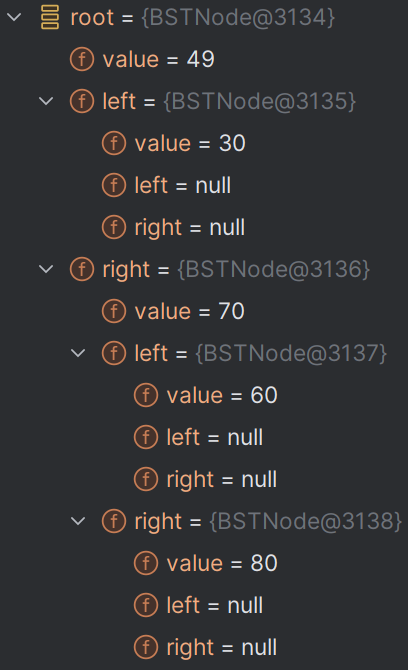
\includegraphics[width=0.475\textwidth]{images/variables.png}
    \caption{Variables during debugging in \intellij}
    \label{fig:variablesIntellij}
\end{figure}

The visual debugger will represent the same information graphically as an object diagram.
Using the visual debugger is \textit{straightforward} since it opens automatically during debugging in the IDE.
The visual debugger visualizes the variables in the scope of the debugging session (see, for example, \autoref{fig:variablesVisualDebugger}) and, stepping through the source code, updates this representation.
\autoref{fig:variablesVisualDebugger} contains the same objects and level of detail as \autoref{fig:variablesIntellij}.
There is a little more debug information in \autoref{fig:variablesIntellij} due to well-written \textsf{toString()} methods which are used by \intellij{}.
In addition, the coloring in \autoref{fig:variablesVisualDebugger} highlights variable changes and additions, a new feature of the visual debugger discussed in \autoref{subsec:improvements}.

\begin{figure}[ht]
    \centering
    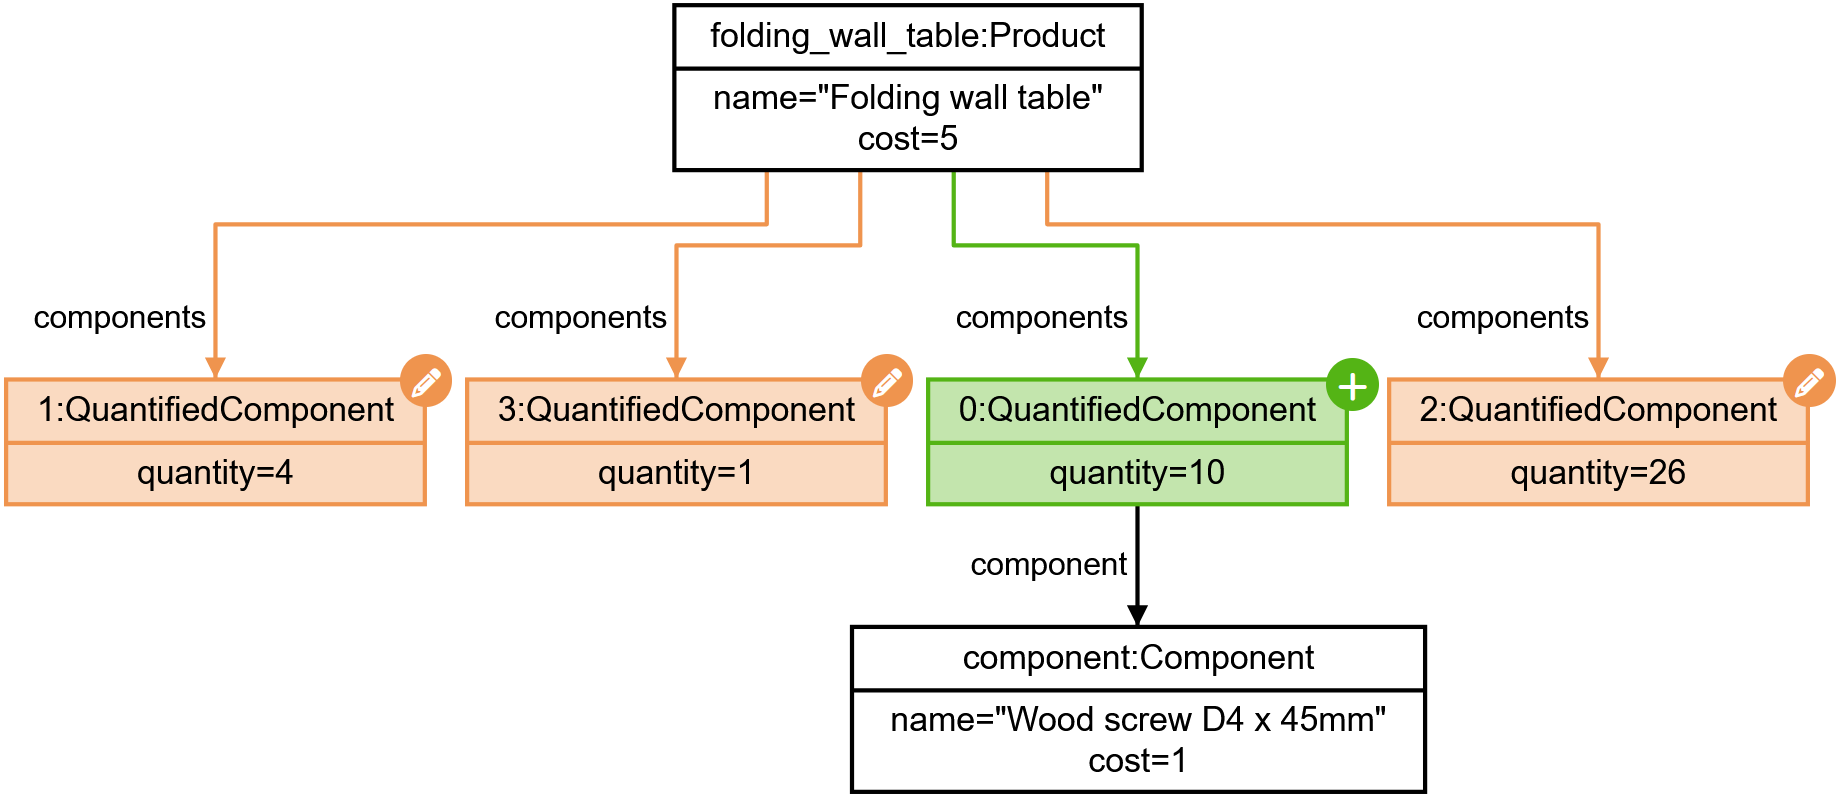
\includegraphics[width=0.475\textwidth]{images/variables-visual-debugger.png}
    \caption{Object diagram of \autoref{fig:variablesIntellij} in the visual debugger}
    \label{fig:variablesVisualDebugger}
\end{figure}

The graphical visualization does not replace the textual debugging view but aims to improve program comprehension during debugging\cite{krauterVisualDebuggerTool2022}.
Concretely, the visual debugger is \textit{non-intrusive} since it can be used alongside the traditional textual debugging available in the IDE.

The visual debugger automatically updates the debug information just as the \intellij{} debugger whenever a user steps through the source code or a new breakpoint is reached.
Moreover, the objects a debugging variable refers to can be loaded by double-clicking an object in the object diagram, similar to how it works in most textual debuggers.
For example, in \autoref{fig:variablesVisualDebugger}, all objects the green object refers to were loaded.
The goal is to make the visual debugger \textit{familiar} by adopting how textual debuggers work such that a transition is smooth.

More information about the visual debugger, including a typical usage scenario, can be found in \cite{krauterVisualDebuggerTool2022}.
% TODO: Make video 2.0 and update link.
In addition, a demonstration of the visual debugger is available at \url{https://www.youtube.com/watch?v=lU_OgotweRk}, and the tool can be installed using \cite{timkrauterVisualDebuggerIntelliJ2023}.

\subsection{Architecture}
In this section, we briefly summarize the architecture of the visual debugger.
The plugin's architecture plays an important role in the improvements and new features of the visual debugger, as well as in understanding the roadblocks we discuss in \autoref{sec:lessonsLearned}.
The visual debugger is separated into two independent components communicating through the \textit{Visual Debugging API} \cite{krauterVisualDebuggerTool2022}.
\autoref{fig:architecture} summarizes the architecture of the visual debugger.

\begin{figure}[ht]
  \centering
  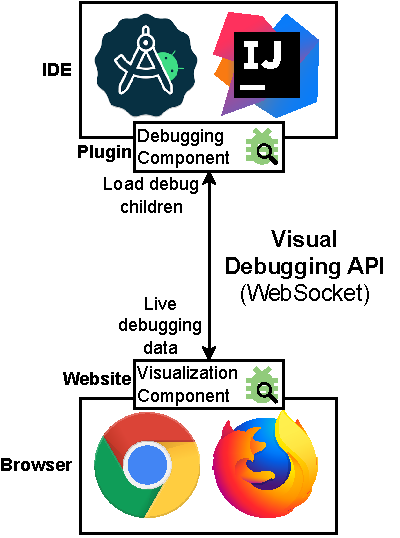
\includegraphics[width=0.65\linewidth]{images/visual-debugger-architecture.pdf}
  \caption{Visual debugger architecture}
  \label{fig:architecture}
\end{figure}

The first component, the \textit{debugging component}, integrates with \intellij{}, and its primary function is to acquire stack frame variables throughout the debugging process repeatably.
The debugging component makes this information available via a WebSocket server that implements our Visual Debugging API.
Upon establishing a connection to the Visual Debugging API, a client receives real-time updates with the latest debugging information and can request to load referenced objects for an existing object.

The second component, the \textit{visualization component}, portrays stack frame variables as an object diagram for better understanding (refer to \autoref{fig:variablesVisualDebugger} for an illustration).
It is implemented using web technologies and our object diagram library \cite{timkrauterObjectdiagramjs2023} to visualize the debug information.
Additionally, it leverages the Visual Debugging API to communicate with the debugging component.
Thus, it is agnostic of the IDE used for debugging and can even be reused for other programming languages than Java/Kotlin.
In practice, the visualization component is hosted on a web server inside the IDE, as part of the visual debugger plugin.

The downside to this flexibility is that the visual debugger is not entirely integrated into \intellij{}, as the visualization occurs in a browser external to the IDE.
The rationale behind opting for this approach instead of native IDE integration is discussed in \autoref{sec:lessonsLearned}.
In addition, the next section discusses recent improvements to the visual debugger, which led to a better IDE integration despite a web-based user interface.

% Improvements would be better loading
\subsection{Improvements \& New Features} \label{subsec:improvements}
We made two major improvements to the visual debugger, optimizing its integration with the IDE and expanding its applicability to more complex debugging scenarios.

\textbf{Improvement (1):} We integrated an embedded browser into the visual debugger panel inside \intellij{}.
The embedded browser uses the Java Chromium Embedded Framework (JCEF), available by default in \intellij{}.
As a result, users now have the option to use the embedded instead of an external browser.
Most of the functionality of our visualization component worked out of the box with the JCEF browser.
Additionally, nearly all other features, for example, exporting object diagrams to XML/SVG, were successfully implemented using JCEF APIs.

The Chromium Embedded Framework (CEF) \cite{marshallgreenblattChromiumEmbeddedFramework2023} is integrated with numerous programming languages, including the Java integration JCEF.
The CEF plays a crucial role in many popular applications, for example, the cross-platform Steam Client\footnote{\url{https://developer.valvesoftware.com/wiki/Chromium_Embedded_Framework}}.
However, integrating web applications into \intellij{} is not entirely seamless, which is also highlighted by the fact that using JCEF is still an experimental feature in \intellij{}.
Consequently, we give each user the choice to use the embedded or external browser.
We discuss the problems we faced using JCEF and possible improvements in \autoref{sec:lessonsLearned}.

\textbf{Improvement (2):} We enhanced the loading mechanism for stack frame variables inside the visual debugger.
Previously, we had to pre-load and cache more debug information than was requested by the user since we could not load debug information on demand.
The initial load invalidated the underlying stack frame supplied by the Java Debugging Interface (JDI).
Now, we leverage the APIs provided by \intellij{}, which are a thin wrapper around the JDI.
This enables us to defer loading additional debug information until explicitly required.
Consequently, there is no longer a need to pre-load potentially unnecessary debug information.
This optimization has improved performance, making the visual debugger applicable to more intricate debugging scenarios.

Furthermore, we enhanced the visual debugger by introducing the following two new features:

% Visualizing changes
\textbf{Feature (1):} The visualization component of the visual debugger now \textit{highlights changes} using colors and overlays in the object diagram.
New objects and links are colored green, while changes to existing elements lead to orange coloring.
Computing and highlighting the changes is enabled by default but can be switched off.
\autoref{fig:variablesVisualDebugger} shows the new change visualization by highlighting three changed, and one added object accordingly.
% Motivation
A software engineer is usually most interested in the changes that occur to the objects during debugging.
Our color-based visualization of changes in the object diagram makes it easier for a software engineer to see changes even when dealing with a complex debugging situation with multiple connected objects.

% Implementation
Changes can be calculated efficiently using unique object IDs provided during debugging.
We implemented the change detection in the visualization component such that it can be reused across programming languages and IDEs \cite{timkrauterICSE2024Artifacts2023}.

% Debug history
\textbf{Feature (2):} Furthermore, the visualization component now keeps a \textit{debug history} so that a user can see debug information from previous debugging steps.
The debug history's length is configurable or can be turned off entirely.
% Motivation
As described earlier, software engineers are most interested in how variables change during debugging.
Consequently, to not only highlight differences to the previous step, we save the previous debugging information in a debug history.
A software engineer can thus inspect the previously shown debug information and step as far back as he configured.
The visual debugger always shows where the debug information was collected in the source code, and highlights changes compared to the previous debugging step.
In addition, one can still export the debug information to an image or even edit it in our object diagram modeler \cite{timkrauterObjectdiagramjs2023} for documentation purposes \cite{krauterVisualDebuggerTool2022}.

% Implementation
We implemented the \textit{debug history} in the visualization component to be independent of the used programming language and IDE.
Thus, both features follow our aim of providing a reusable visualization of the stack frame variables set in our previous publication \cite{krauterVisualDebuggerTool2022}.

\section{Lessons Learned \& Roadblocks} \label{sec:lessonsLearned}
The most important lesson we learned is that more features are available during plugin development than what is documented.
Thus, after a thorough search in the documentation, it is beneficial to ask a question in the community forum for plugin development.
If one asks precise, detailed questions, one receives helpful answers quickly, making the forum an immensely valuable resource.
For example, our new deferred loading of debug information discussed in \autoref{subsec:improvements} was enabled due to the \intellij{} forum.
The forum provides the rare opportunity to interact directly with JetBrains developers.

While developing the visual debugger plugin, we encountered two significant roadblocks.
In the remaining portion of this section, we will describe these roadblocks and how to overcome them in the future.

% Roadblock 1: IDE integration due to IDE UI technology --> See notes --> JCEF
\textbf{Roadblock (1):} Creating a user interface with interactive diagramming capabilities and integrating it into \intellij{} was challenging for different reasons.
The IntelliJ Platform is built on Java, and plugin user interfaces utilize the Swing framework.
However, we could not find a diagramming framework for Swing to implement an interactive object diagram for our visualization component.
\intellij{} uses \textit{yFiles} \cite{yworksYFilesDiagrammingLibrary2023}, for example, to visualize generated class diagrams from source code.
For us, \textit{yFiles} was not an option because the cheapest license already carries a significant cost, and we do not plan to monetize our plugin.

Thus, we started with an embedded visualizer using PlantUML \cite{arnaudroquesPlantUML2023} to generate pictures of object diagrams.
Finally, to allow interactions with object diagrams, we opted for the free and open-source \textit{diagram-js} library to implement our web-based library \textit{object-diagram-js} \cite{timkrauterObjectdiagramjs2023} used in the visual debugger.
To summarize, the rich web ecosystem and its growing popularity among developers have led us to a web-based visualization.
Integrating a web-based user interface into \intellij{} is not obvious compared to other IDEs, such as Visual Studio Code, which is built on web technologies and heavily uses web views for extensions.

To integrate our web-based user interface into \intellij{}, we now use JCEF as described in \autoref{subsec:improvements}.
We were unaware of this possibility for an extended period.
We believe the plugin documentation regarding JCEF and web views has room for improvement to take full advantage of the rich web ecosystem.
First, it should be more visible that the integration of web views is possible.
Second, the integration poses challenges that can be reduced by more extensive documentation about JCEF.
Currently, we are authoring a pull request to improve the plugin documentation, incorporating insights gained from our experience with the visual debugger. % TODO: Do this.

% Roadblock 2: Missing APIs for less popular IDEs.
\textbf{Roadblock (2):} Other IDEs than \intellij{} are missing debugging-related APIs to implement our plugin.
Users of the visual debugger have asked us if the plugin could be adapted to work with other IDEs and programming languages.
For example, we would like to support debugging \textit{Go} applications inside the GoLand IDE.
However, compared to \intellij{} plugins, there is no API to hook into debugging processes in GoLand.
Thus, it is currently not possible to adapt the visual debugger for GoLand such that it seamlessly integrates with the IDE.
Our visualization component cannot operate without a debugging component that provides debugging information from GoLand.
This represents a major roadblock to adopting the visual debugger for other IDEs and programming languages.
One could develop the necessary APIs and debugging components for each desired IDE and programming language combination.
Nevertheless, there would be significant redundancy across all these implementations.

A possible solution would be to utilize the \textit{Debug Adapter Protocol} (DAP) \cite{microsoftDebugAdapterProtocol2023}.
The DAP is a sibling of the more popular \textit{Language Server Protocol} (LSP) \cite{microsoftLanguageServerProtocol2023} and standardizes an abstract protocol for how a development tool communicates with concrete debuggers.
The motivation is that debuggers have to be implemented only once for each language and then can be reused in different IDEs, Editors, or other tools, such as our visual debugger, see \autoref{fig:DAP_Architecture}.
Since not all current debuggers will adopt this protocol, an intermediary component is envisioned to adapt an existing debugger to the DAP \cite{microsoftDebugAdapterProtocol2023}, see \textit{debug adapters} in \autoref{fig:DAP_Architecture}.

\begin{figure}[ht]
  \centering
  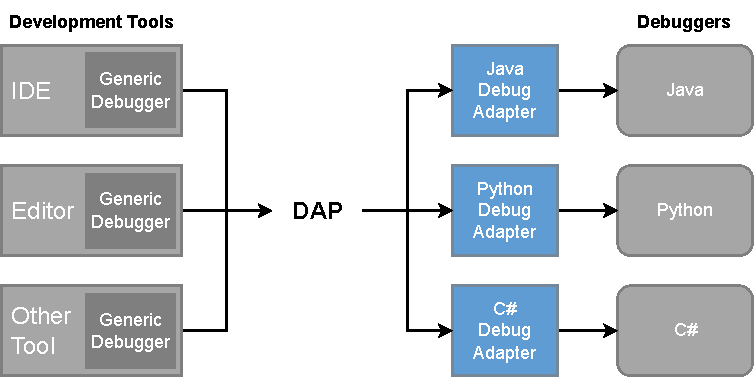
\includegraphics[width=1\linewidth]{images/visual-debugger-DAP-architecture.pdf}
  \caption{Debug Adapter Protocol Architecture \cite{microsoftDebugAdapterProtocol2023}}
  \label{fig:DAP_Architecture}
\end{figure}

Like our visual debugging API, the DAP is independent of development tools (as shown on the left side of \autoref{fig:DAP_Architecture}) and is also language-agnostic (as depicted on the right side of \autoref{fig:DAP_Architecture}).
How JetBrains or other IDEs communicate with its integrated debuggers does not have to use the DAP.
However, each IDE could provide debug adapters for the supported programming languages or integrate existing debug adapters into the IDE.
In addition, using a standard protocol requires minimal documentation and leads to fewer support inquiries.

If the visual debugger also supports the DAP in the future, it can attach to the different debug adapters, which all provide the DAP, i.e., the same interface.
As a result, the visual debugger becomes compatible with any combination of IDE and programming language that provides a debug adapter.
For example, the visual debugger could be automatically available for more IDEs/Editors, such as GoLand (Go), RustRover (Rust), Netbeans (Java), and Visual Studio Code.

After the success of the LSP, it seems like the DAP is on track to become the next standardized development tool functionality \cite{raskVisualStudioCode2020,borkLanguageServerProtocol2023}.
The official page of the DAP lists 11 tools supporting the DAP, 67 debug adapters, and 11 DAP SDKs as of December 2024 \cite{microsoftDebugAdapterProtocol2023}, including, for example, a Go DAP implementation maintained by Google \cite{googleGoImplementationDebug2023}.
Research is also conducted on the DAP to debug Domain-Specific Languages \cite{jeanjeanIDECodeReifying2021,enetProtocolBasedInteractiveDebugging2023}.

\section{Conclusion \& Future work} \label{sec:conclusion}
% Conclusion
The visual debugger has increased in popularity, measured by the more than doubling of downloads of the plugin compared to our previous publication \cite{krauterVisualDebuggerTool2022}.
In this work, we make two contributions related to the visual debugger and the broader topic of IDE integration.

% Summarize improvements and new features
Our first contribution is represented by the improvements and new features we incorporated into the visual debugger.
We have integrated our visual debugger more smoothly into the IDE by employing an embedded browser based on the Java Chromium Embedded Framework (JCEF) and improved the performance of loading debugging information.
Furthermore, the visual debugger now highlights changes graphically using colors and overlays, and we implemented a debug history.

% Summarize roadblocks and their solutions
Our second contribution is detailing the experience gained by implementing the visual debugger.
We described two major roadblocks hampering tighter IDE integration of our plugin.
First, integrating web-based user interfaces that use the extensive and popular web ecosystem is not trivial.
Using the JCEF makes this integration possible, but its visibility and documentation should be improved.
Second, not all IDEs offer debugging-related APIs such that we could integrate our plugin.
To make debugging functionality uniformly accessible for plugin development, we propose to utilize the standardized Debug Adapter Protocol (DAP).

% Future work
In future work, we aim to adapt the visual debugger for other IDEs and code editors such as GoLang, Eclipse \cite{desrivieresEclipsePlatformIntegrating2004}, and Visual Studio Code since this has been requested by our users.
We aim to implement the DAP to minimize the integration effort and development cost for the different IDEs.

Furthermore, it would be interesting to study the usability of the visual debugger and its impact on program comprehension.
It seems interesting to find out in which scenarios visual debugging is more effective than textual debugging and vice versa.
Since the visual debugger is \textit{not} meant to replace the textual debugger, one should also include a combination of both textual and visual debugging in an empirical study.

% Add acknowledgments after review
% \section{Acknowledgments}

\renewcommand\UrlFont{\color{black}}

\bibliographystyle{ACM-Reference-Format}
\bibliography{bib}
\end{document}
